\chapter{Quan sát, vật chất tối và sự khớp của mô hình vũ trụ học}

\lectureoverview{Quan sát chỉ có ý nghĩa sau khi được gắn với một mô hình vũ trụ học. Chúng ta bắt đầu với phương trình Friedmann và ba hình học không gian thuần nhất, sắp xếp ngân sách vũ trụ hiện nay thành bức xạ, vật chất, năng lượng chân không và độ cong, rồi dựng lại vì sao một vũ trụ mở từng có vẻ là điều không thể tránh khỏi. Các đường cong quay của thiên hà sau đó phơi bày phần vật chất hấp dẫn còn thiếu và dẫn tới động lực học của một quầng lạnh, tương tác yếu. Cuối cùng, độ dịch đỏ, độ sáng và số đếm nguồn biến một lịch sử giãn nở giả định thành các đường cong quan sát được. Mô hình cũ chỉ gồm vật chất và độ cong thất bại; một phần vật chất gần \(0.3\), một phần chân không gần \(0.7\), và độ cong rất nhỏ cho ra mô hình khớp thành công được trình bày trong bài giảng.}

\section{Đưa các quan sát trở lại các phương trình}

Không thể diễn giải các dữ kiện thiên văn một cách biệt lập. Trước hết ta cần những phương trình cho biết những tổ hợp quan sát nào phân biệt vũ trụ này với vũ trụ khác. Đối với một vũ trụ đồng nhất và đẳng hướng, điểm xuất phát là phương trình Friedmann,
\begin{equation}
\left(\frac{\dot a}{a}\right)^2
=
\frac{8\pi G}{3}\rho-\frac{k}{a^2}.
\label{eq:c06-friedmann}
\end{equation}
Đại lượng
\begin{equation}
H(t)=\frac{\dot a(t)}{a(t)}
\label{eq:c06-hubble}
\end{equation}
là \emph{hàm} Hubble. Giá trị hiện tại của nó, \(H_0\), theo quy ước được gọi là hằng số Hubble, nhưng \(H(t)\) không hằng trong suốt lịch sử vũ trụ. Khi các nhà thiên văn nêu một giá trị theo đơn vị kilômét trên giây trên megaparsec, họ đang nêu \(H_0\).

Chỉ số độ cong chuẩn hóa chỉ nhận ba giá trị,
\begin{equation}
k\in\{+1,0,-1\},
\end{equation}
lần lượt tương ứng với hình học không gian cầu, phẳng và hyperbolic. Metric FRW quen thuộc có thể được viết
\begin{equation}
ds^2=-dt^2+a(t)^2\left[dr^2+\xi(r)^2d\Omega_2^2\right],
\label{eq:c06-frw}
\end{equation}
trong đó
\begin{equation}
\xi(r)=
\begin{cases}
\sin r, & k=+1,\\
r, & k=0,\\
\sinh r, & k=-1.
\end{cases}
\label{eq:c06-xi}
\end{equation}
Ký pháp này sẽ làm hai việc. Nó gói ba hình học vào một metric, và về sau nó cho diện tích của một mặt cầu, do đó cho số nguồn trong một vỏ cầu theo bán kính. Vì vậy, một lựa chọn \(k\) cùng một phương trình cho \(a(t)\) đã là một mô hình có các hệ quả quan sát được rồi.

\section{Ngân sách vũ trụ hiện nay}

Mật độ năng lượng có ba thành phần chính trong mô hình đang xét: bức xạ, vật chất không tương đối tính và năng lượng chân không. Nếu ghi cả độ cong trên cùng một dòng hạch toán, ta có
\begin{equation}
\frac{C_r}{a^4}
+\frac{C_m}{a^3}
+\Lambda
-\frac{k}{a^2}
=H^2.
\label{eq:c06-budget}
\end{equation}
Ở đây \(\Lambda\) dùng chuẩn hóa của bài giảng trước, \(\Lambda=(8\pi G/3)\rho_{\rm vac}\). Bức xạ bị pha loãng theo \(a^{-4}\), vật chất theo \(a^{-3}\), năng lượng chân không không bị pha loãng, còn độ cong tỉ lệ theo \(a^{-2}\). Độ cong không phải là một mật độ năng lượng vật chất, nhưng đặt nó bên cạnh các hạng khác làm cho ràng buộc hiện tại trở nên minh bạch: bốn đóng góp phải cộng lại thành \(H_0^2\).

Định nghĩa các phần hiện tại của chúng bởi
\begin{equation}
\begin{aligned}
\Omega_r&=\frac{C_r/a_0^4}{H_0^2},
&\qquad
\Omega_m&=\frac{C_m/a_0^3}{H_0^2},\\
\Omega_\Lambda&=\frac{\Lambda}{H_0^2},
&
\Omega_k&=\frac{-k/a_0^2}{H_0^2}.
\end{aligned}
\label{eq:c06-omegas}
\end{equation}
Khi đó
\begin{equation}
\boxed{\Omega_r+\Omega_m+\Omega_\Lambda+\Omega_k=1.}
\label{eq:c06-sum-rule}
\end{equation}
Các \(\Omega\) là những tỉ số được đánh giá tại thời điểm hôm nay, không phải các hằng số bất biến theo thời gian. Cũng lưu ý quy ước dấu: \(k=-1\) cho một \(\Omega_k\) dương.

\subsection{Cách đo các số hạng đầu tiên}

Hubble đã thu được tốc độ giãn nở cục bộ bằng cách so sánh độ dịch đỏ lùi với khoảng cách. Độ dịch đỏ cho một vận tốc ở \(z\) nhỏ; độ sáng đã hiệu chuẩn cho một khoảng cách. Giá trị số đầu tiên của ông sai rất nhiều, nhưng phương pháp thì đúng. Vì các thiên hà ở tương đối gần, phép đo không thăm dò một phần lớn của lịch sử vũ trụ và có thể coi \(H\) là giá trị hiện tại của nó.

\begin{classroomqa}
\audiencequestion{Làm thế nào độ sáng có thể xác định khoảng cách nếu độ sáng nội tại chưa được biết sẵn?}
\lecturerresponse{Điều đó không thể làm được chỉ trong một bước. Thang khoảng cách vũ trụ bắt đầu bằng thị sai đối với các sao gần. Các sao biến quang Cepheid trong vùng đã được hiệu chuẩn đó cho thấy một quan hệ chu kỳ–độ sáng và trở thành các ngọn nến chuẩn cho những khoảng cách lớn hơn. Các phép hiệu chuẩn chồng lấp đưa thang này ra xa dần, và siêu tân tinh cung cấp những ngọn nến tốt nhất ở các độ dịch đỏ vũ trụ học sẽ dùng về sau. Vì vậy khoảng cách được suy ra từ một chuỗi chuẩn, chứ không phải từ một giả định tùy tiện rằng mọi thiên thể đều sáng như nhau. \lecturetimestamp{00:10:00--00:11:32}}
\end{classroomqa}

\begin{classroomqa}
\audiencequestion{Mặc dù mật độ của chúng thay đổi, \(C_r\) và \(C_m\) có phải là các hằng số không?}
\lecturerresponse{Có. Các hệ số vẫn cố định trong khi các thừa số \(a^{-4}\) và \(a^{-3}\) mang sự phụ thuộc theo thời gian. Năng lượng chân không là hằng, còn độ cong tỉ lệ theo \(a^{-2}\). Chính các lũy thừa khác nhau đó là lý do khiến các phần đóng góp tương đối thay đổi từ thời kỳ này sang thời kỳ khác. \lecturetimestamp{00:11:35--00:12:02}}
\end{classroomqa}

Số hạng bức xạ có thể được đo cục bộ từ nền photon. Phần lớn của nó là bức xạ nền vi ba vũ trụ, và mật độ năng lượng hiện nay của nó là rất nhỏ so với các thành phần quan trọng khác. Cần một thể tích lấy trung bình đủ lớn, nhưng không cần khảo sát một quãng dài dọc theo nón ánh sáng quá khứ để xác lập rằng \(\Omega_r\) là không đáng kể ngày nay.

Vật chất khả kiến được ước lượng từ các thiên hà, các quần thể sao, hydro và khí giữa các sao. Các phương pháp này mang tính kỹ thuật hơn là tối nghĩa về mặt khái niệm: xác định lượng sao và khí điển hình, cộng trên các thiên hà, rồi lấy trung bình trên một thể tích lớn. Bài giảng nêu thang xấp xỉ cũ là một khối lượng proton trên mỗi mét khối. Con số này lớn hơn nhiều so với mật độ bức xạ nhưng vẫn loãng đến mức đáng kinh ngạc.

\begin{classroomqa}
\audiencequestion{Còn vật chất tối trong cách hạch toán này thì sao?}
\lecturerresponse{Ta sẽ nói đến nó ngay sau đây, nhưng trước hết chúng ta cố ý dựng lại suy luận cũ chỉ dựa trên vật chất phát sáng. Trật tự lịch sử này rất quan trọng: nó cho thấy chính xác kết luận có vẻ hợp lý nào đã được vật chất tối sửa lại, và khoảng trống nào nó không khép lại. \lecturetimestamp{00:15:08--00:15:40}}
\end{classroomqa}

\section{Vì sao một vũ trụ mở từng có vẻ tất yếu}

Trong bức tranh cũ, bức xạ được đánh giá đúng là không đáng kể, năng lượng chân không được đặt bằng không, và vật chất chỉ có nghĩa là vật chất nhìn thấy được qua bức xạ điện từ. Ước lượng thu được khi đó xấp xỉ là
\begin{equation}
\Omega_r\simeq0,
\qquad
\Omega_\Lambda=0,
\qquad
\Omega_m^{\rm luminous}\sim\frac{1}{20}\text{--}\frac{1}{30}.
\end{equation}
Khi ấy quy tắc tổng dường như buộc
\begin{equation}
\Omega_k\simeq1.
\end{equation}
Vì một đóng góp độ cong dương có nghĩa là \(-k/a_0^2>0\), điều này suy ra \(k=-1\): một vũ trụ mở, có độ cong âm. Những con số này là sự dựng lại lập luận cũ, không phải một ước lượng tham số hiện đại.

Để diễn giải thang độ cong, hãy trở lại nghiệm do vật chất chi phối
\begin{equation}
a(t)\propto t^{2/3}.
\end{equation}
Lấy đạo hàm rồi chia cho \(a\) cho
\begin{equation}
H(t)=\frac{\dot a}{a}=\frac{2}{3t}.
\label{eq:c06-matter-h}
\end{equation}
Ở tuổi hiện tại \(T\),
\begin{equation}
H_0\simeq\frac{2}{3T}.
\end{equation}
Vì vậy thời gian Hubble cùng bậc với tuổi của vũ trụ. Phép so sánh trong trường hợp bức xạ chi phối,
\begin{equation}
a(t)\propto t^{1/2},
\qquad
H(t)=\frac{1}{2t},
\end{equation}
cho thấy quan hệ nghịch với tuổi này không phải là điều riêng của bụi.

\begin{figure}[htbp]
\centering
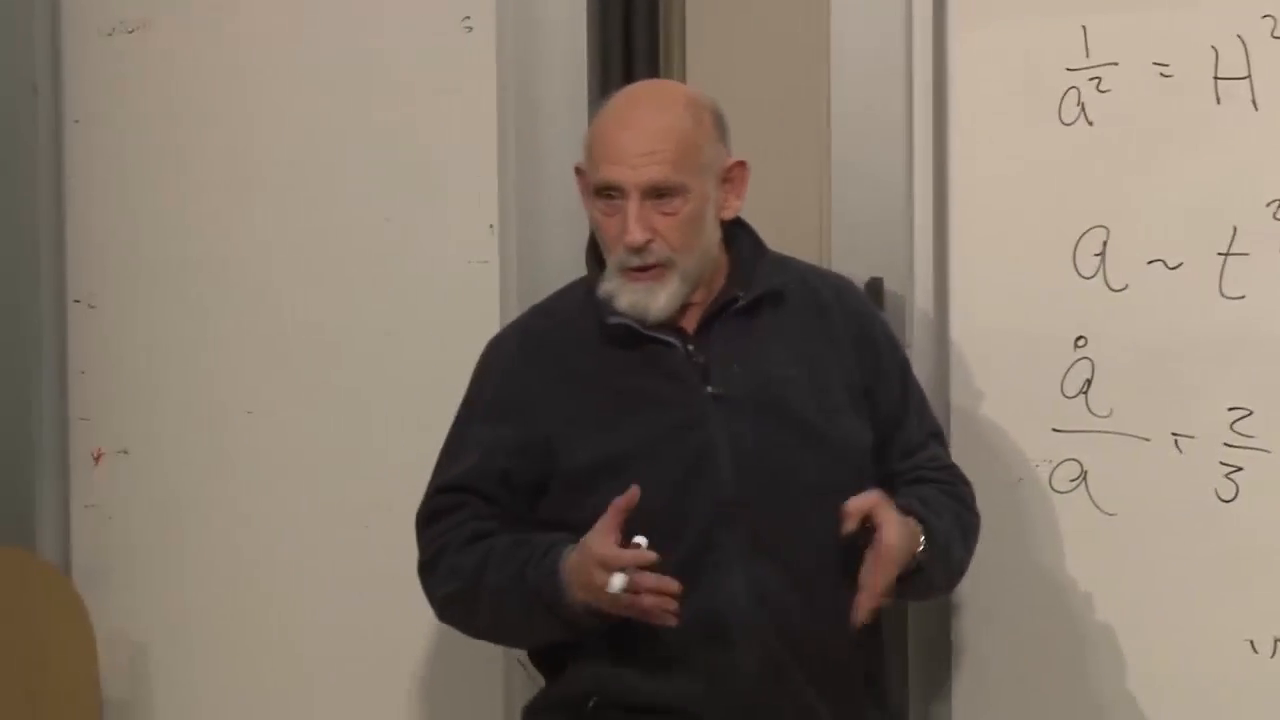
\includegraphics[width=0.72\textwidth]{lecture_06_figure_02.png}
\caption{Ôn lại trên bảng về kỷ nguyên vật chất. Phần chữ nhìn thấy được chứa \(a\sim t^{2/3}\) và \(\dot a/a=2/(3t)\); giảng viên che khuất phần còn lại của bảng, nên không quy cho khung hình bất kỳ phương trình ẩn nào.}
\label{fig:c06-age-board}
\lectureframe{00:24:41.615}
\end{figure}

\begin{classroomqa}
\audiencequestion{Hằng số Hubble có những đơn vị nào, và tốc độ ánh sáng ở đâu?}
\lecturerresponse{Vì \(H\) liên hệ vận tốc với khoảng cách, nó có đơn vị là nghịch đảo thời gian. Nó có thể được nêu theo nghịch đảo giây, nghịch đảo năm, hoặc đơn vị tương đương của giới thiên văn là kilômét trên giây trên megaparsec. Quan hệ \(H\sim1/T\) không cần thêm \(c\). Một thừa số \(c\) chỉ xuất hiện khi thời gian \(T\) được chuyển thành một độ dài như \(cT\). \lecturetimestamp{00:22:50--00:24:25}}
\end{classroomqa}

Giá trị ban đầu của Hubble đối với \(H_0\) lớn quá mức khoảng một bậc độ lớn, nên tuổi Hubble tương ứng quá ngắn, cỡ một tỷ thay vì mười tỷ năm trong phép so sánh làm tròn của bài giảng. Việc hiệu chuẩn tốt hơn đã sửa lại con số đó mà không thay đổi lập luận rằng \(H_0^{-1}\) là một thang thời gian vũ trụ.

Suy luận cũ về độ cong nay viết thành
\begin{equation}
\frac{1}{a_0^2}\sim H_0^2\sim\frac{1}{T^2}.
\end{equation}
Trong đơn vị \(c=1\), khi đó bán kính độ cong \(a_0\) được cho là cùng bậc với tuổi \(T\); khi khôi phục các đơn vị thông thường, nó cùng bậc với \(cT\). Bài giảng lập tức rút lại kết luận này như một phát biểu về vũ trụ thực. Đó là kết luận người ta thu được vài thập kỷ trước sau khi loại bỏ các hạng khi ấy được cho là không đáng kể.

\begin{classroomqa}
\audiencequestion{Nếu ngày nay độ cong được cho là chi phối, tại sao lại dùng định luật do vật chất chi phối \(a\propto t^{2/3}\)?}
\lecturerresponse{Bởi vì vật chất tỉ lệ theo \(a^{-3}\) còn độ cong chỉ tỉ lệ theo \(a^{-2}\). Ở \(a\) nhỏ hơn, vật chất thắng thế. Độ cong chỉ có thể trở nên quan trọng vào giai đoạn muộn, nên sự chi phối của vật chất vẫn mô tả phần lớn lịch sử đã trôi qua và giữ \(H_0\) ở cỡ \(1/T\). Một nghiệm hỗn hợp đầy đủ sẽ hiệu chỉnh hệ số số học, chứ không xóa bỏ lập luận về thang thời gian. \lecturetimestamp{00:49:20--00:50:17}}
\end{classroomqa}

\section{Vật chất tối từ động lực học thiên hà}

Có hai cách mang tính thao tác để kiểm kê vật chất. Một là đếm vật chất phát ra hoặc hấp thụ ánh sáng. Cách kia là suy ra khối lượng từ hấp dẫn. Oort đã phát hiện động lực học thiên hà dị thường vào đầu thập niên 1930, và Zwicky tìm thấy sự chênh lệch khối lượng tương tự trong các cụm thiên hà. Chứng cứ cho thấy vật chất gây hấp dẫn vượt quá vật chất phát sáng. Vật chất tích điện thông thường bức xạ và va chạm; thành phần còn thiếu trước hết được nhận ra nhờ tác dụng hấp dẫn của nó.

\begin{classroomqa}
\audiencequestion{Vật chất phát sáng có bao gồm khí khuếch tán và các hố đen ở tâm không?}
\lecturerresponse{Khí khuếch tán được tính đến chừng nào lượng của nó có thể được suy ra từ hành vi điện từ của nó. Một hố đen siêu khối lượng ở tâm có thể được tính vào ngân sách khối lượng đã biết, nhưng nó chỉ chiếm một phần nhỏ của tổng khối lượng thiên hà và tập trung ở tâm. Nó không thể giải thích một sự sai khác vẫn còn tồn tại ở rất xa bên ngoài vùng tâm phát sáng. \lecturetimestamp{00:29:50--00:31:14}}
\end{classroomqa}

Xét một ngôi sao chuyển động gần đúng trên một quỹ đạo tròn bán kính \(r\). Nếu gần như toàn bộ khối lượng \(M\) tập trung gần tâm thiên hà, thì định luật Newton cho
\begin{equation}
\frac{GM}{r^2}=\frac{v^2}{r},
\end{equation}
và do đó
\begin{equation}
v^2=\frac{GM}{r},
\qquad
v(r)\propto r^{-1/2}.
\label{eq:c06-kepler}
\end{equation}
Đây là quy luật suy giảm kiểu Kepler được kỳ vọng ở bên ngoài một phân bố khối lượng tâm.

\begin{figure}[htbp]
\centering
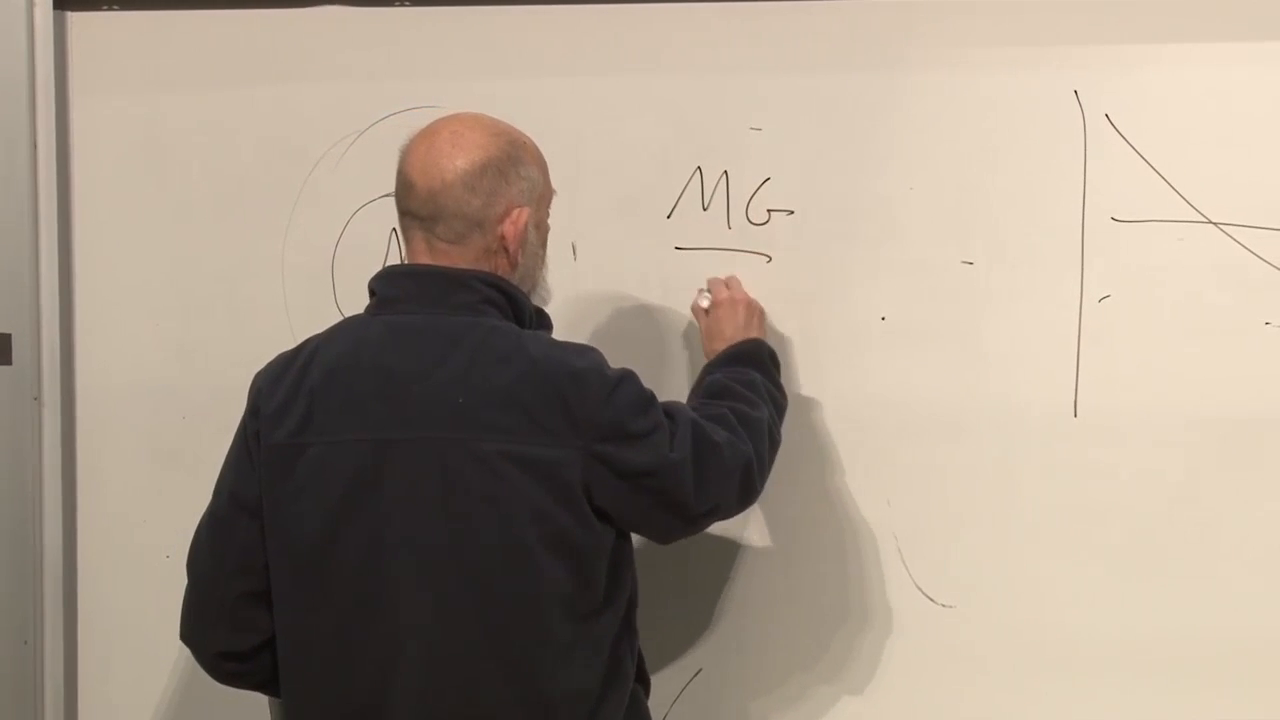
\includegraphics[width=0.78\textwidth]{lecture_06_figure_03.png}
\caption{Bảng về đường cong quay tại chỗ chuyển từ một khối lượng tâm sang khối lượng bao trong \(M(r)\). Chỉ nhìn thấy \(MG\), gạch phân số, phác họa quỹ đạo và các phần của các phác họa đường cong; phương trình~\eqref{eq:c06-kepler} đến từ phần suy diễn bằng lời.}
\label{fig:c06-rotation-board}
\lectureframe{00:34:53.642}
\end{figure}

\begin{figure}[htbp]
\centering
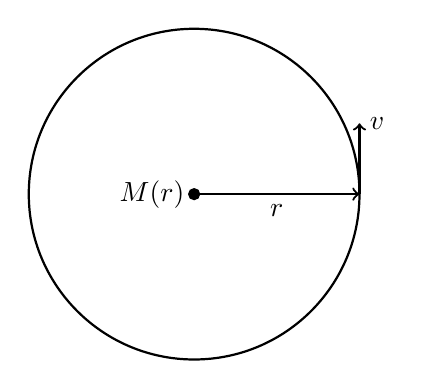
\begin{tikzpicture}[scale=1.0]
\filldraw (0,0) circle (2pt) node[left] {\(M(r)\)};
\draw[thick] (0,0) circle (2.1);
\draw[->,thick] (0,0)--(2.1,0) node[midway,below] {\(r\)};
\draw[->,thick] (2.1,0)--(2.1,0.9) node[right] {\(v\)};
\end{tikzpicture}
\caption{Cấu hình quỹ đạo tròn dùng để suy ra khối lượng bao trong từ tốc độ quay đo được.}
\label{fig:c06-orbit-redraw}
\end{figure}

Đường cong quay thiên hà quan sát được không suy giảm theo cách này; trên một khoảng bán kính đáng kể, chúng gần như phẳng. Thay khối lượng tâm cố định bằng khối lượng bao trong \(M(r)\):
\begin{equation}
\frac{G M(r)}{r^2}=\frac{v(r)^2}{r}.
\end{equation}
Nếu \(v(r)\) gần như không đổi, thì
\begin{equation}
\boxed{M(r)\propto r.}
\label{eq:c06-enclosed-mass}
\end{equation}
Điều này nói về tổng khối lượng bên trong bán kính \(r\), không phải về mật độ cục bộ. Khối lượng gây hấp dẫn tiếp tục tăng ra xa vượt hẳn vùng nơi phần lớn ánh sáng sao tập trung. Các chuyển động vuông góc với đĩa thiên hà còn cho thấy một phân bố gần cầu: một quầng tối chứ không phải một đĩa mỏng thứ hai.

\begin{classroomqa}
\audiencequestion{Có một lý thuyết đơn giản nào giải thích vì sao đường cong quay lại phẳng đến vậy không?}
\lecturerresponse{Không có trong lập luận này. Các mô phỏng về sự hình thành thiên hà có thể khiến những dạng như vậy trở nên tự nhiên, nhưng bài giảng không khẳng định có một phép suy ra ngắn gọn. Phát biểu chắc chắn là phát biểu quan sát: \(v\) gần như không đổi hàm ý khối lượng bao trong tăng gần tuyến tính. Không nên nhầm tính gọn ghẽ của quan hệ đó với một lời giải thích sơ cấp về sự hình thành thiên hà. \lecturetimestamp{00:35:58--00:37:33}}
\end{classroomqa}

\begin{classroomqa}
\audiencequestion{Các cánh tay xoắn ốc có đơn thuần là những chong chóng vật chất do tốc độ góc biến thiên \(v/r\) tạo ra không?}
\lecturerresponse{Không có bức tranh chong chóng đơn giản nào đúng cả. Mẫu hình nhìn thấy không nhất thiết quay cùng các sao riêng lẻ; mô tả bằng sóng mật độ hoặc sóng hình thành sao là những khả năng trong số đó. Bài giảng dùng sự bất định này để tách suy luận vững chắc về quầng ra khỏi bài toán phức tạp hơn về cấu trúc xoắn ốc. \lecturetimestamp{00:37:35--00:38:34; 00:47:03--00:47:47}}
\end{classroomqa}

Khối lượng tối được suy ra lớn gấp vài lần khối lượng phát sáng, và trong bài giảng chỉ được nêu như một hệ số bậc độ lớn vào khoảng từ 5 đến 10. Quầng cũng còn kéo dài ra ngoài thiên hà nhìn thấy được. Đây cố ý là những thang ước lượng lịch sử thô, không phải các tỉ số phổ quát chính xác cho mọi hệ.

\section{Vật chất tối phải có những đặc tính nào}

Vì sao vật chất thông thường tạo thành những đĩa sáng cô đặc, còn vật chất tối vẫn ở trong một quầng rộng? Vật chất phát sáng có thể mất năng lượng cơ học qua va chạm điện từ và bức xạ. Một khi nó tiêu tán năng lượng, lực hấp dẫn có thể kéo nó vào một cấu hình đặc hơn. Vật chất tối dường như trung hòa điện và tương tác yếu hơn nhiều. Các hạt của nó chuyển động theo quỹ đạo trong quầng với rất ít va chạm hay bức xạ, nên ngay cả qua hàng tỷ năm chúng cũng không mất đủ năng lượng để lắng xuống đĩa phát sáng. Bức xạ hấp dẫn từ chuyển động thiên hà quá yếu để cung cấp một cơ chế làm nguội thay thế.

\begin{classroomqa}
\audiencequestion{Việc tương tác rất yếu có nghĩa là vật chất tối tuân theo một định luật hấp dẫn khác sao?}
\lecturerresponse{Không. Người ta giả sử nó hấp dẫn theo cách thông thường. Cụm từ đó ở đây có nghĩa là không có, hoặc bị suy giảm rất mạnh, các va chạm phi hấp dẫn và bức xạ điện từ. Hai hạt tối vẫn hút nhau bằng hấp dẫn; lực hút đó tổ chức nên một quầng nhưng không tiêu tán năng lượng quỹ đạo một cách hiệu quả. \lecturetimestamp{00:42:36--00:43:35}}
\end{classroomqa}

\begin{classroomqa}
\audiencequestion{Những quan sát nào cho thấy đây không chỉ là nét riêng của một đường cong quay thiên hà?}
\lecturerresponse{Bằng chứng xuất hiện ở nhiều thang: chuyển động của sao bên trong thiên hà, chuyển động vuông góc với mặt phẳng thiên hà, tương tác giữa các thiên hà và động lực học của toàn bộ các cụm thiên hà. Các ví dụ của Oort và Zwicky là những biểu hiện khác nhau của cùng một bài toán thiếu hụt hấp dẫn. \lecturetimestamp{00:42:00--00:42:36}}
\end{classroomqa}

\begin{classroomqa}
\audiencequestion{Vật chất tối có tập trung quanh các hố đen và tâm thiên hà không?}
\lecturerresponse{Quả có trở nên đậm đặc hơn về phía một tâm hấp dẫn, nhưng trình tự lịch sử có lẽ ngược với ý tưởng một quầng hình thành quanh một hố đen có sẵn. Các quầng tối đã tạo nên những giếng hấp dẫn lớn; vật chất baryon sau đó rơi vào chúng và hình thành các thiên hà, các sao và các hố đen ở tâm. Hố đen chỉ là một phần nhỏ của khối lượng. Tuy vậy, việc tìm kiếm các sản phẩm hủy cặp vẫn hướng về tâm thiên hà vì mật độ vật chất tối được kỳ vọng là cao hơn ở đó. \lecturetimestamp{00:43:36--00:45:43}}
\end{classroomqa}

\begin{classroomqa}
\audiencequestion{Vật chất tối là khí, bụi, các đám đặc gọn, hay các hạt cô lập? Có thể có một phần bị giữ gần Mặt Trời không?}
\lecturerresponse{Bản chất vi mô của nó chưa biết, nhưng bụi thông thường được liên kết bởi các lực điện từ, đúng kiểu tương tác mà vật chất tối dường như thiếu. Vì thế, bức tranh hạt mặc định là một quần thể loãng gồm các hạt riêng lẻ. Một số có thể bị tập trung bởi hấp dẫn gần Mặt Trời, tuy vậy mật độ của chúng quá nhỏ để cạnh tranh với hấp dẫn của Mặt Trời hoặc gây nhiễu động lực học hành tinh. \lecturetimestamp{00:45:43--00:47:02; 00:58:41--00:59:29}}
\end{classroomqa}

Yêu cầu trung tâm thứ hai là vật chất tối phải kết cụm. Một quần thể nóng với các tốc độ ngẫu nhiên tương đối tính chống lại sự kết tụ hấp dẫn; một quần thể lạnh có thể rơi vào các giếng thế. Các neutrino nhẹ thông thường hẳn sẽ hành xử như vật chất tối nóng và không cung cấp thành phần thiên hà chủ yếu cần có. Trong ngữ cảnh này, \emph{lạnh} có nghĩa là phi tương đối tính trong hệ quy chiếu vũ trụ học địa phương, không phải theo nghĩa đen ở nhiệt độ không của phòng thí nghiệm.

\begin{classroomqa}
\audiencequestion{Yêu cầu phải lạnh để kết cụm có áp đặt một khoảng khối lượng cho vật chất tối không?}
\lecturerresponse{Điều đó phụ thuộc vào thống kê lượng tử và lịch sử sản sinh. Các fermion rất nhẹ không thể tất cả cùng chiếm một trạng thái tốc độ thấp và bị ràng buộc rất mạnh. Các boson rất nhẹ có thể chiếm một trạng thái ngưng tụ Bose kết hợp; axion là ví dụ của bài giảng. Ngoài ra, các hạt nặng hơn tương tác yếu có thể lạnh mà không cần ngưng tụ. Vì thế, lập luận này không cung cấp một cận khối lượng đơn nhất độc lập với mô hình. \lecturetimestamp{00:53:17--00:54:52; 00:56:42--00:58:05}}
\end{classroomqa}

\begin{classroomqa}
\audiencequestion{Các máy gia tốc lẽ ra đã phải tìm ra các hạt ấy rồi sao?}
\lecturerresponse{Chỉ dưới những giả định bổ sung. Nếu các hạt có tiết diện cỡ tương tác yếu và khối lượng nằm trong tầm với của máy gia tốc, thì việc tạo ra chúng trong máy va chạm có thể là khả dĩ. Kỳ vọng của bài giảng rằng thông tin sắp có là điều được nêu rõ là mang tính suy đoán và gắn với bối cảnh lịch sử. Thay vào đó, một hạt có thể quá nặng hoặc tương tác quá yếu đối với các thí nghiệm hiện có. \lecturetimestamp{00:54:52--00:55:54}}
\end{classroomqa}

\begin{classroomqa}
\audiencequestion{Có phải vật chất tối chỉ đơn thuần tồn tại trong một chiều phụ không nhìn thấy?}
\lecturerresponse{Không cần đến một cơ chế như vậy trong phần thảo luận này. Vật chất tối đã được quan sát thông qua hấp dẫn và có thể đơn giản chỉ gồm những hạt khác thường hầu như không tương tác với vật chất thông thường. Gọi một tương tác là yếu không đồng nghĩa với việc đặt các hạt ra ngoài không-thời gian quan sát được. \lecturetimestamp{00:55:54--00:56:41}}
\end{classroomqa}

Việc sửa đổi hấp dẫn thay vì thêm vật chất không nhìn thấy là một phương án hợp logic. Bài giảng cho rằng khi đó không có sửa đổi nào đơn giản tương đương lại giải thích được bằng chứng trên mọi thang liên quan, đồng thời vẫn giữ được các định luật thành công của hệ Mặt Trời. Vì thế cách diễn giải theo hạt được ưa chuộng hơn, nhưng vi vật lý của nó vẫn chưa biết.

\section{Vật chất tối không khép kín ngân sách cũ}

Vật chất tối làm tăng đóng góp của vật chất lên vài lần, nhưng độ chênh cũ giữa vật chất phát sáng và \(H_0^2\) có cỡ 25. Vì thế nó thu hẹp khoảng cách nhưng vẫn không khiến
\begin{equation}
\frac{C_m}{a_0^3}=H_0^2.
\end{equation}
Trong bức tranh cũ không có \(\Lambda\), vẫn cần một số hạng dương trong ngân sách độ cong và do đó cần \(k<0\). Không có gì mâu thuẫn về mặt logic trong một mô hình mở như vậy; điểm mấu chốt là chỉ riêng vật chất tối không tự mình chọn ra đáp án hiện đại.

\begin{classroomqa}
\audiencequestion{Trước phép khớp hiện đại, các nhà vũ trụ học thực sự đã nghĩ gì về độ cong?}
\lecturerresponse{Bằng chứng khi đó khá rối rắm, và sự thiên về trước đó đối với một vũ trụ đóng, hữu hạn đôi khi đi ngược lại ngân sách vật chất. Khi các giả định cũ được kết hợp một cách nhất quán, suy luận tự nhiên là độ cong âm. Sự đồng thuận lịch sử đó vẫn chỉ là tạm thời vì cả vật chất tối lẫn năng lượng chân không đều chưa được đưa vào một cách vững chắc như ngày nay. \lecturetimestamp{00:50:17--00:51:50}}
\end{classroomqa}

Vì vậy, ta phải kiểm định mô hình ứng viên thay vì suy ra rằng nó đúng chỉ từ một hạng mục trong bảng ngân sách. Một mô hình gồm một lựa chọn độ cong \(k\) và một lịch sử giãn nở \(a(t)\), hay tương đương là một tập các phương trình trạng thái của các thành phần và các tham số hiện tại mà từ đó tính được \(a(t)\). Mô hình ứng viên cũ là vật chất cộng với độ cong âm, với bức xạ không đáng kể và không có hằng số vũ trụ.

\section{Biến hình học thành các đại lượng quan sát được}

\subsection{Số đếm nguồn và độ sáng trong một hình học cố định}

Tạm thời bỏ qua sự tiến hóa vũ trụ. Trong một vũ trụ đồng nhất, số nguồn trong một lớp vỏ đồng chuyển động tỉ lệ với diện tích của nó:
\begin{equation}
dN\propto \xi(r)^2\,dr.
\label{eq:c06-shell-count}
\end{equation}
Do đó
\begin{equation}
dN\propto
\begin{cases}
\sin^2r\,dr, & k=+1,\\
r^2\,dr, & k=0,\\
\sinh^2r\,dr, & k=-1.
\end{cases}
\end{equation}
Ở \(r\) lớn, trường hợp độ cong âm tăng như \(\sinh^2r\sim e^{2r}\), nhanh hơn rất nhiều so với định luật phẳng \(r^2\). Vì thế, độ cong âm dự đoán số lượng nguồn tăng nhanh bất thường theo khoảng cách.

Chính diện tích ấy cũng chi phối thông lượng thu được. Trong không gian tĩnh phẳng, một nguồn chuẩn cho
\begin{equation}
F\propto\frac{1}{r^2}.
\end{equation}
Trong không gian hyperbolic, mặt cầu mà trên đó bức xạ lan ra tăng nhanh hơn, nên thông lượng giảm nhanh hơn. Bài giảng đôi khi gọi đại lượng quan sát này là độ sáng; ở đây \(F\) ký hiệu độ sáng biểu kiến hoặc thông lượng, còn độ sáng nội tại thuộc về nguồn. Vì vậy, số đếm và độ sáng khi xét cùng nhau có thể phân biệt các hình học không gian.

\subsection{Độ lệch đỏ và nón ánh sáng quá khứ}

Vũ trụ thực sự có tiến hóa, và nhìn ra xa có nghĩa là nhìn ngược về thời gian. Ánh sáng phát ra tại \(t_{\rm em}\) bị kéo giãn khi thừa số tỉ lệ tăng từ \(a(t_{\rm em})\) lên \(a_0\):
\begin{equation}
1+z
=\frac{\lambda_{\rm obs}}{\lambda_{\rm em}}
=\frac{a_0}{a(t_{\rm em})}.
\label{eq:c06-redshift}
\end{equation}
Tương đương,
\begin{equation}
z=\frac{\lambda_{\rm obs}}{\lambda_{\rm em}}-1.
\end{equation}
Các điểm khác nhau dọc theo nón ánh sáng quá khứ của chúng ta đồng thời tương ứng với các bán kính đồng chuyển động khác nhau và các thời điểm phát xạ khác nhau. Sự giãn nở làm thay đổi bước sóng; dịch chuyển Doppler và dịch chuyển hấp dẫn là những cơ chế vật lý khác, nhưng hiệu ứng được xét ở đây là sự giãn nở vũ trụ.

\begin{classroomqa}
\audiencequestion{Vì sao định nghĩa của \(z\) lại chứa trừ một?}
\lecturerresponse{Đó là một quy ước lịch sử, được chọn sao cho một nguồn không bị dịch chuyển có \(z=0\). Hệ số kéo giãn trực tiếp về mặt vật lý là \(1+z=\lambda_{\rm obs}/\lambda_{\rm em}\). \lecturetimestamp{01:10:11--01:10:45}}
\end{classroomqa}

Ánh sáng theo phương bán kính có \(d\Omega_2=0\) và tuân theo \(ds^2=0\). Vì vậy, phương trình~\eqref{eq:c06-frw} cho
\begin{equation}
dt^2=a(t)^2dr^2.
\end{equation}
Đối với một tia tới được lần ngược từ phía chúng ta,
\begin{equation}
dt=-a(t)\,dr,
\qquad
\frac{dr}{dt}=-\frac{1}{a(t)}.
\label{eq:c06-null-ray}
\end{equation}
Dấu trừ cho biết bán kính đồng chuyển động lớn hơn nằm ở thời điểm sớm hơn dọc theo tia. Một khi \(a(t)\) đã biết, phương trình này xác định \(r(t)\).

\subsection{Số lượng trên mỗi đơn vị độ lệch đỏ}

Người quan sát có thể đếm các nguồn chuẩn trong một khoảng độ lệch đỏ từ \(z\) đến \(z+dz\). Bắt đầu từ phương trình~\eqref{eq:c06-shell-count} và vi phân phương trình~\eqref{eq:c06-redshift} dọc theo tia sáng trong nón ánh sáng quá khứ:
\begin{equation}
dz=-\frac{a_0}{a^2}\,da
=-\frac{a_0}{a^2}\dot a\,dt.
\end{equation}
Dùng \(dt=-a\,dr\),
\begin{equation}
dz=\frac{a_0}{a}\dot a\,dr
=(1+z)\dot a\,dr.
\end{equation}
Do đó
\begin{equation}
dr=\frac{dz}{(1+z)\dot a},
\end{equation}
và, với mật độ nguồn đồng chuyển động cố định,
\begin{equation}
\boxed{
\frac{dN}{dz}
\propto
\frac{\xi(r)^2}{(1+z)\dot a}
}.
\label{eq:c06-dndz}
\end{equation}
Trong phần suy dẫn trực tiếp trên lớp, các dấu và hệ số được kiểm tra hơn một lần; các phương trình~\eqref{eq:c06-null-ray} và \eqref{eq:c06-redshift} xác định kết quả một cách không mơ hồ.

\begin{figure}[htbp]
\centering
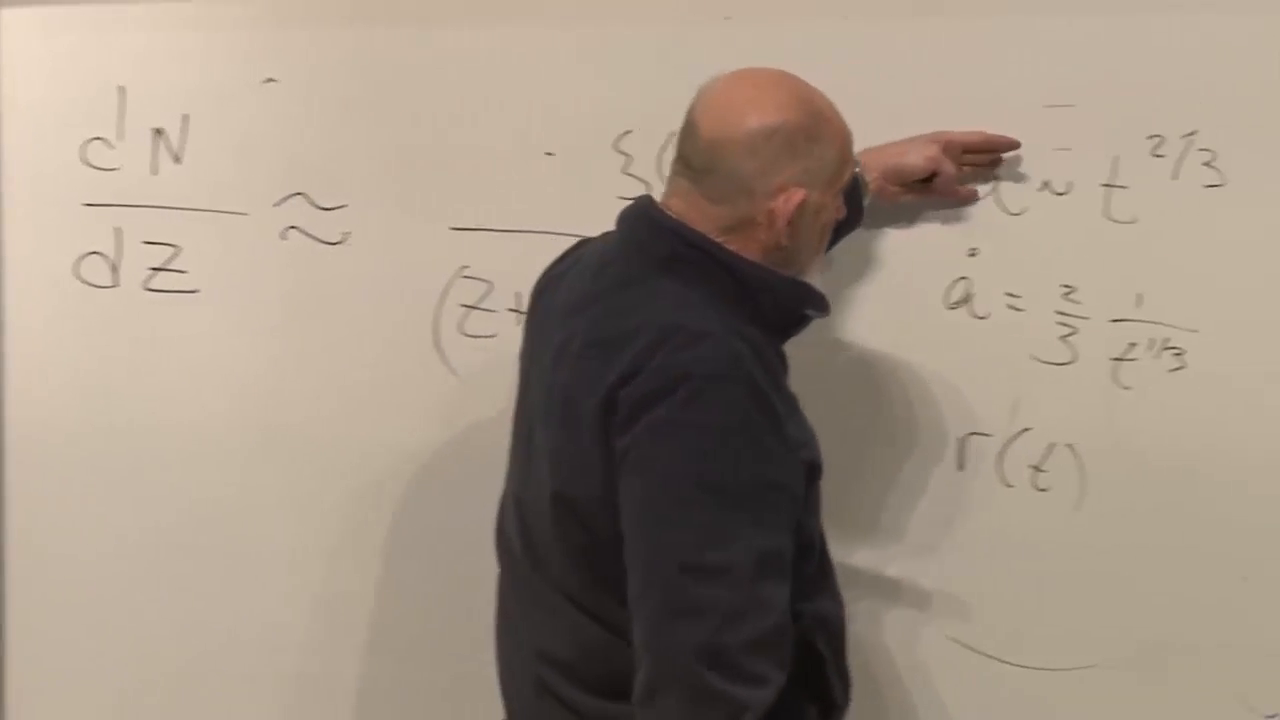
\includegraphics[width=0.84\textwidth]{lecture_06_figure_05.png}
\caption{Quan hệ trên bảng giữa \(dN/dz\) và các hàm của mô hình. Vế trái và \(a\sim t^{2/3}\), \(\dot a\), và \(r(t)\) ở vế phải đều nhìn thấy được, còn giảng viên che khuất một phần mẫu số; phương trình~\eqref{eq:c06-dndz} đã được thiết lập độc lập ở phía trên.}
\label{fig:c06-dndz-board}
\lectureframe{01:22:24.114}
\end{figure}

Không còn gì để tính tiếp cho đến khi một mô hình được chọn. Một \(a(t)\) cho trước quyết định \(\dot a(t)\), phương trình~\eqref{eq:c06-null-ray} quyết định \(r(t)\), và phương trình~\eqref{eq:c06-redshift} cho phép biểu diễn mọi đại lượng theo \(z\). Các phương trình trạng thái khác nhau tạo ra các hàm \(dN/dz\) và \(F(z)\) khác nhau. Chính điều này làm cho các quan sát có khả năng phân biệt.

\section{Từ các tham số thử đến phép khớp tốt nhất}

Quy trình là trực tiếp:
\begin{equation}
(\Omega_r,\Omega_m,\Omega_\Lambda,\Omega_k)
\longrightarrow
a(t)
\longrightarrow
\left\{F(z),\frac{dN}{dz}\right\}.
\label{eq:c06-fit-pipeline}
\end{equation}
Chọn các tham số hiện tại, giải phương trình Friedmann, cho ánh sáng truyền theo phương bán kính, tính độ sáng và số đếm theo độ lệch đỏ, rồi so sánh các đường cong với dữ liệu. Nếu so sánh thất bại thì bác bỏ bộ tham số đó. Gộp lại, hai đại lượng quan sát này ràng buộc cả lịch sử giãn nở lẫn hình học không gian.

\begin{figure}[htbp]
\centering
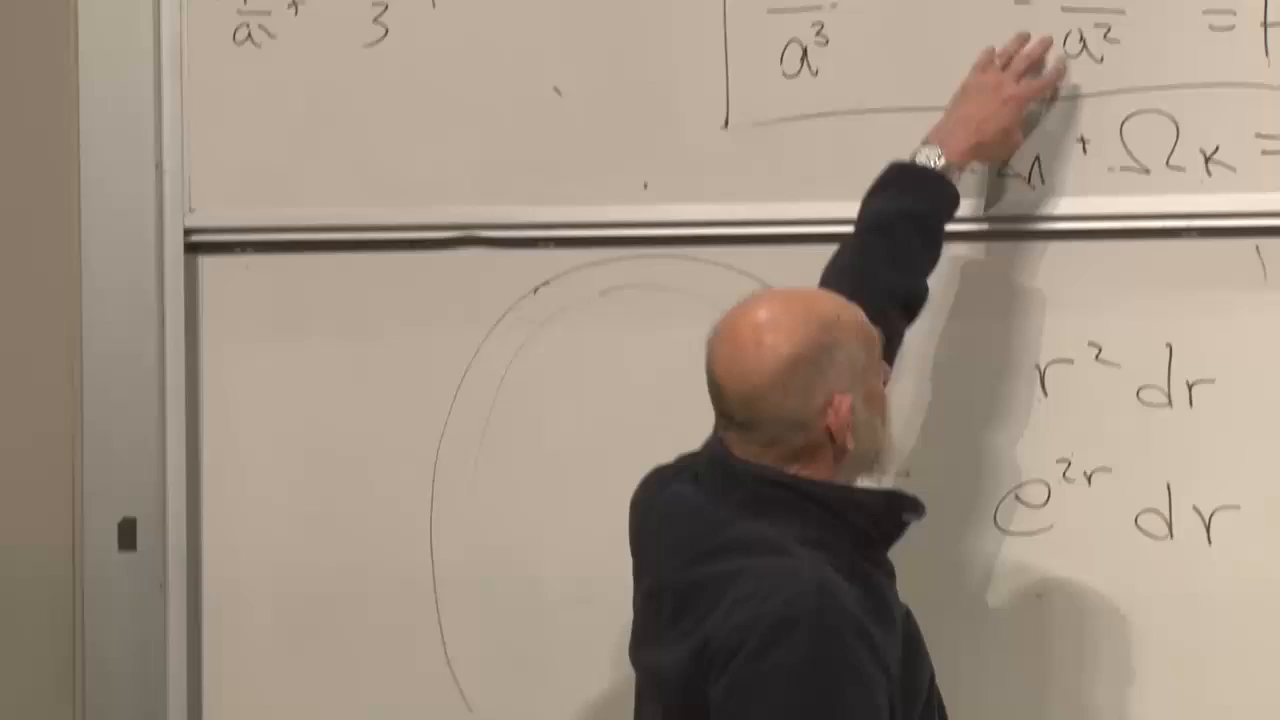
\includegraphics[width=0.84\textwidth]{lecture_06_figure_06.png}
\caption{Mô hình cũ gồm vật chất cộng độ cong trên phần bảng phía trên, và các thừa số lớp vỏ phẳng và hyperbolic \(r^2dr\) và \(e^{2r}dr\) trên phần bảng phía dưới. Một số phần của phương trình Friedmann bị che khuất, nên khung hình này là bằng chứng hỗ trợ chứ không phải nguồn của phương trình.}
\label{fig:c06-old-model-board}
\lectureframe{01:24:27.863}
\end{figure}

Mô hình cũ,
\begin{equation}
H^2=\frac{C_m}{a^3}-\frac{k}{a^2},
\qquad k=-1,
\end{equation}
không phù hợp cả với quan hệ độ sáng-độ lệch đỏ lẫn phép kiểm tra số đếm nguồn. Các siêu tân tinh cung cấp những nến chuẩn hữu ích nhất trong dải độ lệch đỏ liên quan. Bộ tham số thành công trong bài giảng là
\begin{equation}
\boxed{
\Omega_r\simeq0,\qquad
\Omega_m\simeq0.3,\qquad
\Omega_\Lambda\simeq0.7,\qquad
\Omega_k\simeq0
}.
\label{eq:c06-best-fit}
\end{equation}
Ở đây vật chất bao gồm cả vật chất sáng lẫn vật chất tối. Các giá trị này phản ánh phép khớp ở thời kỳ của bài giảng; bài học bền vững là phương pháp khớp và sự cần thiết của một thành phần trội không bị pha loãng, chứ không phải chữ số thập phân cuối cùng được in ra.

\subsection{Các câu hỏi về điều gì được đo và điều gì được khớp}

\begin{classroomqa}
\audiencequestion{Liệu \(\Lambda\) đã được giả định sẵn khi mô hình vũ trụ mở cũ đang được thảo luận hay chưa?}
\lecturerresponse{Không. Phần đầu cố ý dựng lại mô hình cũ hơn với \(\Lambda=0\). Các giá trị trong phương trình~\eqref{eq:c06-best-fit} mô tả phép khớp hiện đại về sau. Mô hình ứng viên cũ không bị sửa đổi ngầm; nó đã được kiểm tra với \(F(z)\) và \(dN/dz\) rồi thất bại. \lecturetimestamp{01:26:45--01:27:07}}
\end{classroomqa}

\begin{classroomqa}
\audiencequestion{Làm thế nào thu được \(\Omega_\Lambda\) nếu năng lượng chân không không được đo trực tiếp như vật chất cục bộ?}
\lecturerresponse{Hãy bắt đầu với các bộ tham số thử. Mỗi bộ xác định một nghiệm Friedmann và do đó xác định các hàm dự đoán \(F(z)\) và \(dN/dz\). So sánh các dự đoán ấy với quan sát, loại bỏ các phép khớp kém, và giữ lại miền tốt nhất của không gian tham số. Con số \(0.7\) là một suy luận từ phép khớp, không phải số đọc trực tiếp từ một máy đo năng lượng chân không. \lecturetimestamp{01:27:08--01:29:59; 01:31:57--01:33:40}}
\end{classroomqa}

\begin{classroomqa}
\audiencequestion{Thang hiện tại \(a_0\) đến từ đâu?}
\lecturerresponse{Việc chuẩn hóa \(a\) một phần là quy ước, nhưng một mô hình hoàn chỉnh gắn với \(H_0\) cung cấp thang độ cong vật lý hiện tại khi \(k\ne0\). Một khi mô hình khớp với các đại lượng quan sát theo độ lệch đỏ, hàm \(a(t)\) của nó xác định điểm hiện tại và thang tương ứng. \lecturetimestamp{01:29:59--01:30:42}}
\end{classroomqa}

\begin{classroomqa}
\audiencequestion{Việc nhìn lùi hàng tỉ năm về quá khứ có làm méo một phép khớp dựa trên các tham số ngày nay không?}
\lecturerresponse{Sự nhìn lùi đó không phải là méo dạng; nó chính là tín hiệu. Các tham số ngày nay được đưa vào phương trình Friedmann, phương trình này tiến hóa chúng thành một \(a(t)\) hoàn chỉnh. Nón ánh sáng dự đoán đã bao gồm thực tế là vật chất quan trọng hơn ở \(a\) nhỏ hơn, và nếu đi đủ xa về quá khứ thì bức xạ chi phối. Một mô hình bỏ qua sự tiến hóa này sẽ không khớp dữ liệu. \lecturetimestamp{01:30:43--01:31:55}}
\end{classroomqa}

\begin{classroomqa}
\audiencequestion{Những đại lượng hiện tại nào được đo một cách tương đối trực tiếp?}
\lecturerresponse{Mật độ bức xạ được đo và hiện nay là không đáng kể. Tốc độ Hubble được đo từ quan hệ khoảng cách-độ lệch đỏ. Tổng mật độ vật chất được suy ra bằng hấp dẫn, bao gồm cả vật chất sáng và vật chất tối, rồi chia cho thang tới hạn \(3H_0^2/(8\pi G)\) để thu được \(\Omega_m\). Bậc tự do còn lại ở thời muộn chủ yếu nằm ở năng lượng chân không và độ cong. \lecturetimestamp{01:33:40--01:35:32}}
\end{classroomqa}

\begin{classroomqa}
\audiencequestion{Nếu cả \(\Omega_\Lambda\) lẫn \(\Omega_k\) đều chưa biết, vì sao sau khi cố định \(\Omega_m\) lại chỉ còn một tham số thử độc lập ở thời muộn?}
\lecturerresponse{Vì phương trình~\eqref{eq:c06-sum-rule} áp đặt một ràng buộc. Khi \(\Omega_r\) không đáng kể và \(\Omega_m\) đã được đo, việc chọn một \(\Omega_\Lambda\) thử sẽ cố định phần còn lại \(\Omega_k=1-\Omega_m-\Omega_\Lambda\). Ta cũng có thể tham số hóa cùng họ một chiều ấy bằng độ cong. Chẳng hạn, \(\Omega_\Lambda=0.4\) và \(\Omega_k=0.3\) là một phép thử hợp lệ khi \(\Omega_m=0.3\); nó chỉ bị bác bỏ vì các đường cong dự đoán của nó khớp kém, chứ không phải vì quy tắc tổng cấm nó. \lecturetimestamp{01:35:33--01:39:09}}
\end{classroomqa}

\begin{classroomqa}
\audiencequestion{Làm sao \(k\) chỉ có thể là \(+1,0,-1\) trong khi \(\Omega_k\) biến thiên liên tục, và các thứ nguyên có đúng không?}
\lecturerresponse{Giá trị rời rạc \(k\) chỉ ghi lại dấu và hình học đã chuẩn hóa. Bán kính độ cong liên tục được mang bởi \(a_0\), nên \(-k/(a_0^2H_0^2)\) có thể nhận một dải liên tục các giá trị. Trong hệ đơn vị \(c=1\), nghịch đảo độ dài và nghịch đảo thời gian có cùng thứ nguyên; khi khôi phục các đơn vị thông thường, ta có các lũy thừa cần thiết của \(c\). \lecturetimestamp{01:39:10--01:40:07}}
\end{classroomqa}

\begin{classroomqa}
\audiencequestion{Phương pháp đếm có giả định tính đồng nhất và đẳng hướng hay không, mặc dù các quần thể thiên hà có tiến hóa?}
\lecturerresponse{Nó giả định tính đồng nhất và đẳng hướng theo không gian trên những lát cắt không gian đủ lớn, và có thể kiểm tra các đối xứng đó bằng cách so sánh các hướng khác nhau tại cùng một độ dịch đỏ. Sự tiến hóa của các nguồn là một vấn đề riêng: các quần thể ở những thời kỳ khác nhau không nhất thiết phải giống hệt nhau, nên các phân tích thực tế mô hình hóa hiệu ứng chọn lọc và sự tiến hóa thay vì giả vờ rằng mật độ số là cố định vĩnh viễn. Phép suy diễn đơn giản tách riêng nhân tố hình học trước khi bổ sung các tinh chỉnh đó. \lecturetimestamp{01:40:08--01:41:08}}
\end{classroomqa}

\section{Sự tiến hóa của các tỷ phần mật độ}

Phương trình~\eqref{eq:c06-budget} đúng ở mọi thời điểm, nhưng các \(\Omega\) trong phương trình~\eqref{eq:c06-omegas} được định nghĩa tại thời điểm hiện tại. Các đại lượng tương tự phụ thuộc thời gian ấy biến thiên vì bốn số hạng có các lũy thừa khác nhau của \(a\). Trong quá khứ rất xa,
\begin{equation}
\Omega_r(t)\longrightarrow1.
\end{equation}
Vì bức xạ bị pha loãng nhanh hơn, vật chất dần tiến tới chỗ chiếm ưu thế. Về sau, bản thân vật chất cũng bị pha loãng, còn \(\Lambda\) thì không đổi, nên trong tương lai rất xa,
\begin{equation}
\Omega_\Lambda(t)\longrightarrow1.
\end{equation}
Vì vậy, tỷ phần vật chất ban đầu nhỏ, trở nên gần bằng đơn vị trong thời đại vật chất, rồi lại giảm sau khi năng lượng chân không chiếm ưu thế. Độ cong, nếu khác không, rốt cuộc cũng bị một hằng số dương \(\Lambda\) áp đảo.

\begin{classroomqa}
\audiencequestion{Một tỷ phần độ cong hiện tại nhỏ có nghĩa là vũ trụ trở nên phẳng hơn khi giãn nở không?}
\lecturerresponse{Thang độ cong vật lý của nó tăng theo \(a\), và so với một hằng số vũ trụ dương thì đóng góp độ cong \(a^{-2}\) ngày càng kém quan trọng. Đó là ý nghĩa của cụm \emph{lớn thì phẳng}. Điều đó không làm thay đổi nhãn tôpô rời rạc \(k\); nó nói rằng độ cong cục bộ và tầm quan trọng động lực học theo tỷ phần của độ cong đều giảm. \lecturetimestamp{01:47:13--01:47:42}}
\end{classroomqa}

\begin{classroomqa}
\audiencequestion{Mô hình được khớp có cho thấy các phần dư hệ thống chưa giải thích được không, và tuyên bố ấy chính xác đến mức nào?}
\lecturerresponse{Bài giảng cho biết ở mức đó chưa có sự thất bại hệ thống nào đã biết của khuôn khổ này, và mô tả đây là vũ trụ học chính xác với độ chính xác xấp xỉ cỡ phần trăm, chứ không phải ở mức một phần mười hay một phần trăm của một phần trăm. Phát biểu đó mang tính lịch sử và không nên biến thành một thanh sai số hiện hành như thể đúng cho mọi thời điểm. \lecturetimestamp{01:45:40--01:46:19}}
\end{classroomqa}

\begin{classroomqa}
\audiencequestion{Có thể kiểm tra độ cong không gian bằng phép tam giác đạc trực tiếp thay vì chỉ bằng độ sáng và số đếm siêu tân tinh không?}
\lecturerresponse{Có. Mẫu hình góc của bức xạ nền vi sóng vũ trụ cung cấp một thang vật lý chuẩn và do đó một tam giác vũ trụ lớn. Chỉ riêng dữ liệu siêu tân tinh không cung cấp phát biểu đầy đủ của bài giảng về độ cong ở mức phần trăm; việc kết hợp chúng với hình học của bức xạ nền vi sóng đã làm phép kiểm định sắc nét hơn. Đây là chủ đề của bài giảng tiếp theo. \lecturetimestamp{01:46:19--01:47:12}}
\end{classroomqa}

\section{Điều cần ghi nhớ}

Bài học cốt lõi không phải là một danh sách bốn con số. Nó là một phương pháp. Một bộ tham số vũ trụ học cho ra \(a(t)\); khi đó metric dự đoán sự truyền của ánh sáng, độ sáng của nguồn và số đếm nguồn. Sự phù hợp ấy kiểm định cả các tham số đã chọn lẫn khuôn khổ Friedmann nối chúng lại với nhau. Không có lý do gì khiến một bộ tùy ý phải khớp.

Mô hình cũ với vật chất phát sáng và độ cong âm đã thất bại. Vật chất tối đã sửa lại bảng kiểm kê vật chất hấp dẫn nhưng tự nó vẫn không khép kín được ngân sách Friedmann cũ. Phép khớp thành công vào thời kỳ của bài giảng đòi hỏi xấp xỉ
\begin{equation}
\Omega_m\simeq0.3,
\qquad
\Omega_\Lambda\simeq0.7,
\qquad
\Omega_k\simeq0,
\end{equation}
và độ chính xác trong việc xác định độ cong phụ thuộc quan trọng vào bức xạ nền vi sóng vũ trụ. Mô hình đáng tin vì nhiều quan sát độc lập được quy về một lý thuyết động lực học duy nhất và cùng hội tụ vào một miền của không gian tham số.
